\documentclass[a4paper,12pt]{article}

%% Language and font encodings
\usepackage[english]{babel}
\usepackage[utf8x]{inputenc}
\usepackage[T1]{fontenc}

%% Sets page size and margins
\usepackage[a4paper,top=3cm,bottom=2cm,left=3cm,right=3cm,marginparwidth=1.75cm]{geometry}

%% Useful packages
\usepackage{titling}
\usepackage{amsmath}
\usepackage{graphicx}
\usepackage{hyperref}
\usepackage{fancyhdr}
\graphicspath{{graphics/}}
\pagestyle{fancy}


\lhead{Climate App}
\rhead{Instructions}


\title{\vspace{-2.0cm}Climate App instructions\vspace{-2.0cm}}
\date{\today}
\begin{document}

\maketitle
\thispagestyle{fancy}

\begin{figure}[h]
  \centering
  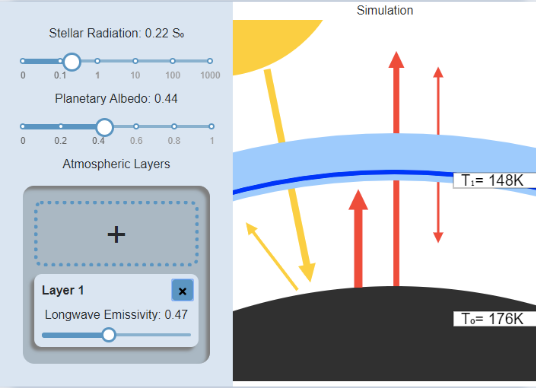
\includegraphics[width=90mm]{demo}
  \caption{Screenshot of the application}
  \label{fig:demo}
\end{figure}

\section*{What is this ?}

This is a web application that is used to demonstrate the effects of greenhouse gases on the temperature of a planet. By choosing the value of different setting shown in the options panel, the user can see a visual representation of the effect on the radiation and temperature. 

\section*{How does it work ?}

\subsection*{Left Panel}

This panel lets you specify values for the settings of the system.

\subsubsection*{Stellar Radiation}

Also known as "Insolation", this value is the amount of radiation from the star that reaches the planet. The units of this measure are "S0", which is the amount of solar radiation on earth. For example, a value of 2 would mean that the planet receives twice the amount of stellar radiation that we have on earth. The slider is a log scale, which allows for value as high as 1000 S0 and as low as 0.01 S0.


\subsubsection*{Planetary albedo}

You can use this slider to choose how reflective the planet is. A value of 1 would mean that the planet reflects all the incoming radiation. A value of zero would mean that the planet is very dark and it absorbs all the incoming radiation. The default value is set to the earth's albedo, which is 0.3

\subsubsection*{Atmospheric Layers}

In this box, you will find settings for the atmospheric layers. You can click the "+" box to add a new layer, and the "x" on a layer to remove it. For each layer, you can set the value of emissivity, which is its effectiveness in emitting energy as thermal radiation. A value of zero would mean that the energy that radiates from the surface entirely goes through the atmospheric layer. A value of one would mean that all of the radiation is absorbed by the layer. A maximum of three layers is possible.

\subsection*{Right Panel}

In this panel, we can see a visual representation of the system. The yellow arrows represent the shortwave emissivity, and the red arrows represent the longwave emissivity. By modifying the input variables, it is possible to see the arrows' size varying in real time.

Please note that the effect of the stellar radiation on the radiation is not represented on the arrow. The reason is that since the insolation is a log scale, if we try to include that setting in the width of the arrows, all the other modification (albedo and emissivity of the layers) would have negligible effects and there would be no visible variation. The arrow size is then proportional to the radiation that they illustrate, assuming constant stellar radiation.

Since there would be a lot of arrows between each layer (see figure \ref{fig:model}), the display of the layers is abstracted in a thick pale blue line. We can still see each layer inside, and their thickness is proportional to their emissivity, but the radiation between themselves is not shown. The resulting temperatures are shown at the surface and at each layer.

\begin{figure}[h]
  \centering
  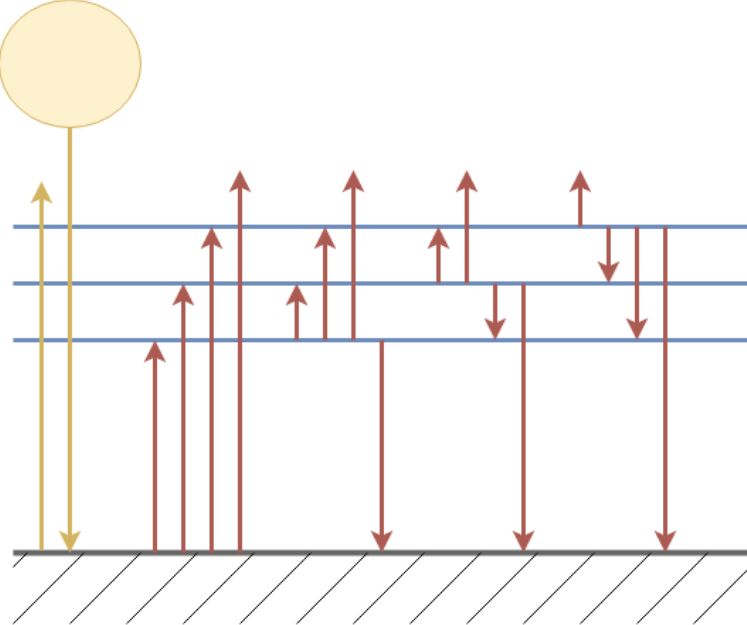
\includegraphics[width=90mm]{Model}
  \caption{}
  \label{fig:model}
\end{figure}

\section*{Why does it work ?}

There are two concepts that we need to be familiar with to understand how to derive the equations:



\subsection*{Stefan-Boltzmann Law}

The Stefan-Boltzmann gives a relation between the temperature of an object and the amount of energy it radiates.

\begin{equation}
    j=\epsilon \sigma T^4
\end{equation}

where $\epsilon$ is the emissivity (We assume $\epsilon = 1$ at the surface), $T$ is the temperature in Kelvin, $j$ is the total energy radiated and $\sigma$ is the Stefan-Boltzmann constant:

\begin{equation*}
    \sigma=5.6703 \times 10^{-8}\ watt/m^2 K^4
\end{equation*}

\subsection*{Radiative equilibrium}

The amount of incoming radiation at any given layer must be equivalent to the outgoing radiation at that layer

\subsection*{Deriving the equations}

Figure \ref{fig:model} gives an illustration of the model that we are analyzing. At the surface, there is incoming stellar radiation, and some of it is reflected back into space (We assume atmospheric layers have no impact on shortwave radiation), as shown by the yellow arrows. The surface then heats and radiates back. Some of this radiation is absorbed by each of the three atmospheric layers, and some of it also makes it into space. The same effect happens for each layer: they heat and then radiates back, both towards space and back to the surface of the planet.

For the surface, using the Stefan-Boltzmann law, we know that the energy radiated is $\sigma T_0^4$, where $T_0$ is the temperature of the surface (Remember that we assume that the planet is a blackbody, that is: $\epsilon_0=1$). According to the radiative equilibrium, if the surface of the planet emits that much radiation, it is because it has absorbed this much. We know that the planet absorbs energy from the star and from each layer. We can then write the following equation:

\begin{equation}
    S_0(1-\alpha)+\epsilon_1 \sigma T_1^4 + \epsilon_2 \sigma T_2^4(1-\epsilon_1)+\epsilon_3\sigma T_3^4 (1-\epsilon_2) (1-\epsilon_1) = \sigma T_0^4
\end{equation}

where $S_0$ is the stellar radiation, $T_i$ and $\epsilon_i$ are the temperature and emissivity at atmospheric layer $i$ respectively, $i=0$ being the surface. The first term is the stellar radiation that is not reflected, and other terms are the radiation that the surface receives from each layer. We can also find those values using the Stefan-Boltzmann law multiplied by the amount of radiation that goes through the other layers.\newline

In a similar fashion, it is possible to get equations for each layer, taking into account that the radiation is emitted both upward and downward:\newline

Layer 1:
\begin{equation}
    \epsilon_1 \sigma T_0^4 + \epsilon_1 \epsilon_2 \sigma T_2^4 +\epsilon_1 \epsilon_3 \sigma T_3^4 (1-\epsilon_e) = 2 \epsilon_1 \sigma T_1^4
\end{equation}

Layer 2:
\begin{equation}
    \epsilon_2 \sigma T_0^4 (1-\epsilon_1) + \epsilon_2 \epsilon_1 \sigma T_1^4 + \epsilon_2 \epsilon_3 \sigma T_3^4 = 2\epsilon_2 \sigma T_2^4
\end{equation}

Layer 3:
\begin{equation}
    \epsilon_3 \sigma T_0^4 (1-\epsilon_1) (1-\epsilon_2) + \epsilon_3 \epsilon_1 \sigma T_1^4(1-\epsilon_2)+\epsilon_3\epsilon_2\sigma T_2^4 = 2 \epsilon_3 \sigma T_3^4
\end{equation}

\subsection*{Solving the equations}

We now have a system of 4 equations and 4 unknown temperature. Solving the system for the fourth power of the temperature yields the following results:\newline

Surface:
\begin{equation}
    T_0^4=\frac{2S_0(\alpha-1)(4-\epsilon_1 \epsilon_2 - \epsilon_1 \epsilon_3 - \epsilon_2 \epsilon_3 + \epsilon_1 \epsilon_2 \epsilon_3)}{\sigma(\epsilon_1-2)(\epsilon_2-2)(\epsilon_3-2)}
\end{equation}

Layer 1:
\begin{equation}
    T_1^4=\frac{S_0(\alpha-1)(4+2\epsilon_2 -2\epsilon_1 \epsilon_2 + 2\epsilon_3 - 2\epsilon_1 \epsilon_3 -3 \epsilon_2 \epsilon_3 + 2\epsilon_1 \epsilon_2 \epsilon_3)}{\sigma(\epsilon_1-2)(\epsilon_2-2)(\epsilon_3-2)}
\end{equation}

Layer 2:
\begin{equation}
    T_2^4=\frac{S_0(\alpha-1)(-2-\epsilon_3+\epsilon_2\epsilon_3)}{\sigma(\epsilon_2-2)(\epsilon_3-2)}
\end{equation}

Layer 3:
\begin{equation}
    T_3^4 = \frac{S_0(\alpha-1)}{\sigma(\epsilon_3-2)}
\end{equation}

Those are the equations that are used in the application to predict the temperature of the system with the given input variables.

\end{document}